\subsection{交互效应面板模型}
\sourcepages{Lecture1-10.pdf, page 41, with the matrix intuition on page 40}
考虑交互效应面板模型
\[
 Y_{it}=A_{i\cdot}B_{t\cdot}^{\mathsf T}+W_{it}\tau+\varepsilon_{it},
 \qquad\mathbb E[\varepsilon\mid A,B,W]=0,\tag{8.5}
\]
其中 $A\in\mathbb R^{n\times k}$、$B\in\mathbb R^{T\times k}$，$k$ 是秩参数。等价地，
\[
 Y_{it}=L_{it}+W_{it}\tau+\varepsilon_{it}
 \qquad\text{对某个秩为 $k$ 的矩阵 }L.
\]
\paragraph{我在左页的矩阵直觉。}
将 $A$ 的取值沿行往下放，$B$ 的取值沿列横向放。秩为一时，交点的元素就是 $a_i b_t$；若 $k\ne1$，则该元素是一个和 $a_{i1}b_{t1}+a_{i2}b_{t2}+\cdots$。\begin{center}\begin{tikzpicture}[>=Stealth,font=\small]
\node at(0,2){$A$};\node at(3,3){$B$};
\node(a)at(0,0){$a_i$};\node(b)at(3,2){$b_t$};\node(p)at(3,0){$a_i b_t$};
\draw[->](a)--(p);\draw[->](b)--(p);
\node[align=center]at(3,-1){当 $k>1$ 时：$\sum_{j=1}^k a_{ij}b_{tj}$};
\end{tikzpicture}\end{center}

处理这个模型，可以考虑合成控制和合成双重差分。假设当且仅当 $i>n_0$ 且 $t>T_0$ 时，$W_{it}=1$。图中在第 $n_0$ 行、第 $T_0$ 列分割结果矩阵，只有右下角区块接受处理。
\begin{center}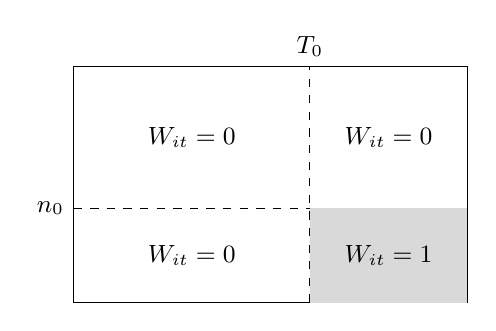
\begin{tikzpicture}[font=\small]
\draw(0,0)rectangle(5,3);\draw[dashed](3,0)--(3,3);\draw[dashed](0,1.2)--(5,1.2);
\fill[black!15](3,0)rectangle(5,1.2);
\node[above]at(3,3){$T_0$};\node[left]at(0,1.2){$n_0$};
\node at(4,.6){$W_{it}=1$};\node at(1.5,2.1){$W_{it}=0$};
\node at(4,2.1){$W_{it}=0$};\node at(1.5,.6){$W_{it}=0$};
\end{tikzpicture}\end{center}


用未处理个体拟合处理组在处理前的轨迹：
\[
 \sum_{i=1}^{n_0}\gamma_iY_{it}
 \approx\alpha+\frac1{n-n_0}\sum_{i=n_0+1}^nY_{it},
 \qquad t=1,\ldots,T_0.
\]
\inkred{第一组从不接受处理；第二组在 $T_0$ 之后接受处理。}截距 $\alpha$ 的作用类似于固定效应。权重选择为
\begin{align*}
 (\widehat\gamma,\widehat\alpha)\in
 \operatorname*{arg\,min}_{\gamma',\alpha}\quad&
 \left\|\sum_{i=1}^{n_0}\gamma'_iY_{i,1:T_0}
 -\frac1{n-n_0}\sum_{i=n_0+1}^nY_{i,1:T_0}
 -\alpha\mathbf1\right\|_2^2,\\
 \text{约束为}\quad&\sum_{i=1}^{n_0}\gamma'_i=1,
 \qquad\gamma'_i\ge0.\tag{8.7}
\end{align*}
\inkred{$\gamma_i$ 的目的是创造平行趋势，从而平衡潜在的 $A_i$ 项。}

最后，在加权的双向模型中估计处理系数：
\[
 (\widehat\tau,\widehat\alpha,\widehat\beta)
 \in\operatorname*{arg\,min}_{\tau',\alpha',\beta'}
 \sum_{i,t}\gamma_i
 (Y_{it}-\alpha'_i-\beta'_t-W_{it}\tau')^2,\tag{8.8}
\]
其中，对 $i>n_0$，$\gamma_i=1/(n-n_0)$。
\notearrow{red}{加权回归中处理个体的权重（第 41 页）}{\inkred{对 $i>n_0$，$\gamma_i=1/(n-n_0)$。}}
处理系数的闭式解为
\begin{align*}
 \widehat\tau={}&\frac1{n-n_0}\sum_{i=n_0+1}^n
 \left\{\frac1{T-T_0}\sum_{t=T_0+1}^TY_{it}
 -\frac1{T_0}\sum_{t=1}^{T_0}Y_{it}\right\}\\
 &-\sum_{i=1}^{n_0}\gamma_i
 \left\{\frac1{T-T_0}\sum_{t=T_0+1}^TY_{it}
 -\frac1{T_0}\sum_{t=1}^{T_0}Y_{it}\right\}.
\end{align*}
\inkred{红色页边批注写道：这依赖 $T_0$ 和 $n$。}在适当的大面板渐近框架下，$n_0,n_1,T\to\infty$ 时，估计量一致。这句话下方还有一条手写限定，但被扫描页底截断；可见部分涉及 (8.5) 的设定以及渐近正态推断，无法恢复完整句子。
\begin{reviewnote}{qualification}{S1-033}{潜在因子平衡与面板渐近条件}{Lecture1-10.pdf, pp. 40, 41}
仅仅在处理前拟合得好，不能证明处理后的反事实趋势已平衡：处理前因子必须揭示处理后相关的方向，还需控制噪声与权重集中程度。该分解的秩至多为 $k$；恰好为 $k$ 还要求因子满秩。一致性结论依赖适当的渐近框架和假设，并非只要 $n,T\to\infty$ 就成立。完整的 synthetic-DID 方法还可能使用时间权重与正则化。参见 \href{https://www.aeaweb.org/articles?id=10.1257/aer.20190159}{Arkhangelsky 等（2021）}及讲义 (8.7)--(8.9)；这里没有根据参考文献补写被截断的原文。
\end{reviewnote}


\paragraph{左页补记。}
合成控制并非处理交互式固定效应的唯一方法。例如，通过 $k$-均值聚类矩阵 $Y$ 的行，然后分别为每个群组拟合时变基线模型。旁边简记“p66，文献”[页码／参考不清楚]。

\subsection{通过可交换性识别}
\sourcepages{Lecture1-10.pdf, page 43, with the extension on page 42}
回顾 $Y_{it}=Y_{it}(0)+W_{it}\tau$。一个基于设计的假设为
\[
 Y_{i\cdot}(0)\perp W_{i\cdot}\mid S_i,
 \qquad S_i=\sum_{t=1}^TW_{it}.\tag{8.10}
\]
其一个推论：考虑线性估计量
\[
 \widehat\tau=\sum_{i,t}\gamma_{it}Y_{it},\tag{8.11}
\]
权重矩阵只依赖 $W$。在 (8.10) 下，给定同一个 $S_i$ 值，未处理潜在结果可交换，并且
\[
 \mathbb E[\widehat\tau\mid W,\gamma]
 =\sum_{i,t}\gamma_{it}\mathbb E[Y_{it}(0)\mid S_i]
 +\tau\sum_{i,t}\gamma_{it}W_{it}.
\]
因此，只要满足下列条件，就可得无偏性：
\[
 \sum_{i,t}\gamma_{it}W_{it}=1,
 \qquad
 \sum_{i:S_i=s}\gamma_{it}=0
 \quad\text{对每个 }t\text{ 和 }s\in\mathcal S,
\]
其中 $\mathcal S$ 是 $S_i$ 的支持集。\notearrow{red}{同一层内，条件期望为常数（第 43 页）}{$\sum_{i:S_i=s}\gamma_{it}=0$ 消去 $\sum_i\gamma_{it}E[Y_{it}(0)\mid S_i]$。}
\begin{reviewnote}{qualification}{S1-034}{个体间可交换性与方差准则}{Lecture1-10.pdf, pp. 42, 43}
要实现上述消去，需要不同个体具有共同的条件均值 $E[Y_{it}(0)\mid S_i=s]=m_t(s)$，以及诸如各行 IID 的条件，保证在给定整张处理分配矩阵时，不会获得超出该个体自身处理路径的额外信息。仅有每一行内给定 $S_i$ 后 $Y_i(0)$ 与 $W_i$ 独立，并不保证个体间可交换性。若约束可行，合并后的限制给出所述双重稳健性。对条件不相关、同方差的各单元，最小化 $\sum_{it}\gamma_{it}^2$ 等于最小化方差；若个体内协方差为 $\Sigma_i$，方差准则应为 $\sum_i\gamma_i'\Sigma_i\gamma_i$。可行权重的无偏性不要求这个工作方差模型正确。
\end{reviewnote}


在这些无偏性约束下，选择使方差最小的 $\gamma$：
\begin{align*}
 \gamma\in\operatorname*{arg\,min}_{\gamma'}\quad&\sum_{i,t}(\gamma'_{it})^2,\\
 \text{约束为}\quad&\sum_{i,t}\gamma'_{it}W_{it}=1,
 \quad\sum_{i:S_i=s}\gamma'_{it}=0\quad\text{对所有 }s,t.\tag{8.14}
\end{align*}
\inkblue{大致说，需要相同 $S_i$ 的个体之间存在 $W_{it}$ 的变异。}

\paragraph{左页扩展：两组识别约束。}
回顾双向模型
\[
 Y_{it}=\alpha_i+\beta_t+W_{it}\tau+\varepsilon_{it},
 \qquad\mathbb E[\varepsilon\mid\alpha,\beta,W]=0.\tag{8.2，回顾}
\]
在这个模型下，若满足下列条件，估计量 (8.11) 也无偏：
\[
 \sum_t\gamma_{it}=0\ \text{对每个 }i,
 \qquad\sum_i\gamma_{it}=0\ \text{对每个 }t,
 \qquad\sum_{i,t}\gamma_{it}W_{it}=1.
\]
\inkred{前两个等式消去固定效应 $\alpha_i$ 和 $\beta_t$，第三个等式将处理系数归一化。}

合并这些约束可得到双重稳健估计量：最小化 $\sum_{i,t}\gamma_{it}^2$，约束为
\[
 \sum_{i,t}\gamma_{it}W_{it}=1,
 \qquad\sum_{i:S_i=s}\gamma_{it}=0\quad\text{对所有 }s,t,
\]
\[
 \sum_t\gamma_{it}=0\quad\text{对所有 }i,
 \qquad\sum_i\gamma_{it}=0\quad\text{对所有 }t.
\]
只要 (8.2) 或 (8.10) 任一成立，它就无偏。补充页顶部附近的简略参考写着“p67，[2019]”[无法从扫描完整识别该引用]。

\section{第 9 讲：工具变量回归}
\sourcepages{Lecture1-10.pdf, page 45, with the three IV conditions on page 44}
工具变量回归处理内生的处理效应问题，即 $Y_i(0)$ 与 $W_i$ 相互依赖的情形。

\subsection{结构模型}
从常数效应模型开始：
\[
 Y_i(w)=Y_i(0)+w\tau,\qquad Y_i=Y_i(W_i).\tag{9.1}
\]
通常，无混杂性指 $\{Y_i(w)\}\perp W_i$；在 (9.1) 中，它就是 $Y_i(0)\perp W_i$。将模型改写为
\notearrow{black}{常数效应潜在结果与无混杂性（第 45 页）}{$Y_i=\alpha+W_i\tau+\varepsilon_i$。}

\[
 Y_i=\alpha+W_i\tau+\varepsilon_i,\tag{9.2}
\]
其中 $\alpha=\mathbb E[Y_i(0)]$，$\varepsilon_i=Y_i(0)-\mathbb E[Y_i(0)]$。在无混杂性下，$\mathbb E[\varepsilon_i\mid W_i]=0$，因此将 $Y_i$ 对 $W_i$ 作 OLS 回归即可估计 $\tau$。

存在混杂时，式 (9.2) 仍成立，但 $\mathbb E[\varepsilon_i\mid W_i]\ne0$。此时 OLS 的目标为
\begin{align*}
 \tau_{\mathrm{OLS}}
 &=\frac{\operatorname{Cov}(Y_i,W_i)}{\operatorname{Var}(W_i)}\\
 &=\frac{\operatorname{Cov}(\tau W_i+\varepsilon_i,W_i)}{\operatorname{Var}(W_i)}
 =\tau+\frac{\operatorname{Cov}(\varepsilon_i,W_i)}{\operatorname{Var}(W_i)}
 \ne\tau.
\end{align*}
\inkred{这个比值被划线标为 OLS 系数。}
\begin{reviewnote}{qualification}{S1-035}{依赖关系未必产生非零线性偏差}{Lecture1-10.pdf, pp. 45}
精确恒等式 $\tau_{\rm OLS}=\tau+\operatorname{Cov}(\varepsilon,W)/\operatorname{Var}(W)$ 是正确的。但 $Y(0)$ 与 $W$ 依赖，未必意味着条件误差均值或协方差非零。例如，$Y(0)$ 的方差可以依赖处理，但条件均值保持不变。所示 $\ne\tau$ 描述的是协方差非零的混杂情形，并非任何依赖关系都会导致这一结论。后面用 IV 比值识别，还需要分母非零。
\end{reviewnote}


\subsection{利用工具变量识别}
引入 $Z_i$：
\[
 Y_i=\alpha+W_i\tau+\varepsilon_i,\qquad\varepsilon_i\perp Z_i,
 \qquad W_i=Z_i\gamma+\eta_i.\tag{9.4}
\]
由于 $Z_i$ 与 $\varepsilon_i$ 不相关，
\[
 \operatorname{Cov}(Y_i,Z_i)
 =\operatorname{Cov}(\tau W_i+\varepsilon_i,Z_i)
 =\tau\operatorname{Cov}(W_i,Z_i).
\]
因此
\[
 \tau=\frac{\operatorname{Cov}(Y_i,Z_i)}{\operatorname{Cov}(W_i,Z_i)},
 \qquad
 \widehat\tau=\frac{\widehat{\operatorname{Cov}}(Y_i,Z_i)}
 {\widehat{\operatorname{Cov}}(W_i,Z_i)}.
\]

\paragraph{我在左页列出的 IV 条件。}
\begin{enumerate}
 \item \textbf{外生性：}$\varepsilon_i\perp Z_i$。
 \item \textbf{相关性：}$\operatorname{Cov}(W_i,Z_i)\ne0$。
 \item \textbf{排除限制：}$Z_i$ 对 $Y_i$ 的所有影响都必须经过 $W_i$。
\end{enumerate}
\begin{center}\begin{tikzpicture}[>=Stealth,font=\small]
\node(z)at(0,0){$Z_i$};\node(w)at(2,0){$W_i$};\node(y)at(4,0){$Y_i$};
\draw[->,red](z)--(w);\draw[->,red](w)--(y);
\draw[->](w) to[bend right=45]node[below]{其他处理影响路径}(y);
\end{tikzpicture}\end{center}

\subsection{最优工具变量}
\sourcepages{Lecture1-10.pdf, page 47, with extensions on page 46 and the estimating-equation reminder on page 48}
允许工具变量 $Z_i\in\mathcal Z$ 为高维：
\[
 Y_i=\tau W_i+\varepsilon_i,\qquad\varepsilon_i\perp Z_i,
 \qquad Y_i,W_i\in\mathbb R.
\]
对函数 $w:\mathcal Z\to\mathbb R$，
\[
 \tau=\frac{\operatorname{Cov}(Y_i,w(Z_i))}
 {\operatorname{Cov}(W_i,w(Z_i))},\tag{9.8}
\]
其中分母非零。哪个变换 $w(\cdot)$ 最优？估计量为
\begin{align*}
 \widehat\tau_w
 &=\frac{\widehat{\operatorname{Cov}}(Y_i,w(Z_i))}
 {\widehat{\operatorname{Cov}}(W_i,w(Z_i))}\\
 &=\frac{n^{-1}\sum_i(Y_i-\overline Y)(w(Z_i)-\overline{w(Z)})}
 {n^{-1}\sum_i(W_i-\overline W)(w(Z_i)-\overline{w(Z)})},\tag{9.9}
\end{align*}
其中 $\overline Y=n^{-1}\sum_iY_i$，其他均值类似定义。它求解以下估计方程：
\[
 \frac1n\sum_i(w(Z_i)-\overline{w(Z)})
 \{Y_i-\overline Y-\widehat\tau_w(W_i-\overline W)\}=0.\tag{9.10}
\]
原稿写为
\[
 n(\widehat\tau_w-\tau)\Rightarrow\mathcal N(0,V_w),
 \qquad
 V_w=\frac{\operatorname{Var}(\varepsilon_i)\operatorname{Var}(w(Z_i))}
 {\operatorname{Cov}(W_i,w(Z_i))^2}.\tag{9.11，原稿缩放}
\]
\begin{reviewnote}{original}{S1-036}{IV 的正态极限需要根号 n 缩放}{Lecture1-10.pdf, pp. 47, 48}
正确极限是 $\sqrt n(\widehat\tau_w-\tau)\Rightarrow N(0,V_w)$。一阶展开为
\[
\sqrt n(\widehat\tau_w-\tau)=
\frac{n^{-1/2}\sum_i(w(Z_i)-E[w(Z)])\varepsilon_i}
{\operatorname{Cov}(W,w(Z))}+o_p(1),
\]
这里要求误差已中心化、观测 IID、所需矩有限，且极限协方差非零。在 $\varepsilon\perp Z$ 下，由此得到所示的 $V_w$。可对照官方讲义 (9.12)；其公式编号与手写笔记不同。
\end{reviewnote}



由于 $Z_i\perp\varepsilon_i$ 且 $\mathbb E[\varepsilon_i]=0$，
\[
 \operatorname{Var}\{\varepsilon_i(w(Z_i)-\mathbb E[w(Z_i)])\}
 =\operatorname{Var}(\varepsilon_i)\operatorname{Var}(w(Z_i)).
\]
笔记写出的优化问题是
\notearrow{red}{使用方差相关比值的倒数（第 47 页）}{下方原稿中求 $w^*(\cdot)$ 的优化问题。}

\[
 w^*(\cdot)\in\operatorname*{arg\,min}_{w'}
 \frac{\operatorname{Cov}(W_i,w'(Z_i))^2}{\operatorname{Var}(w'(Z_i))}.
\]
给出的解为
\[
 w^*(z)\propto\mathbb E[W_i\mid Z_i=z].
\]
\notearrow{red}{$w^*(z)\propto E[W_i\mid Z_i=z]$（第 47 页）}{\inkred{用 $Z_i$ 对 $W_i$ 的最佳预测。}}
\begin{reviewnote}{original}{S1-037}{应最大化协方差比值}{Lecture1-10.pdf, pp. 47}
最小化 $V_w$ 需要
\[
\arg\max_w\frac{\operatorname{Cov}(W,w(Z))^2}{\operatorname{Var}(w(Z))}.
\]
记 $m(Z)=E[W\mid Z]$，由条件期望和 Cauchy--Schwarz 不等式，$\operatorname{Cov}(W,w)^2=\operatorname{Cov}(m,w)^2\le\operatorname{Var}(m)\operatorname{Var}(w)$。在 $\operatorname{Var}(m)>0$ 时，取 $w=a+bm$、$b\ne0$ 可达等号。因此，最佳预测的直觉正确，但优化方向写反了。该结果使用原稿中误差独立于工具变量、相应条件同方差的设定，并非一般异方差情况下的最优工具变量公式。参见官方讲义 (9.13)--(9.15)。
\end{reviewnote}



\paragraph{左页扩展：以协变量为条件。}
\begin{inkblock}{red}
条件可拓展为 $\varepsilon_i\perp Z_i\mid X_i$，得到
\[
 \tau(x)=\frac{\operatorname{Cov}(Y_i,w(Z_i)\mid X_i=x)}
 {\operatorname{Cov}(W_i,w(Z_i)\mid X_i=x)}.
\]
批注提到：构建平均效应 $\tau=\mathbb E[\tau(X)]$ 的双重稳健估计量，以及 $\tau(\cdot)$ 的随机森林估计量。
\end{inkblock}

\begin{reviewnote}{qualification}{S1-038}{条件 IV 比值识别的是什么}{Lecture1-10.pdf, pp. 46}
在条件结构模型 $Y=a(X)+W\tau(X)+\varepsilon$ 下，若 $E[\varepsilon\mid Z,X]=0$ 且条件第一阶段协方差非零，该比值等于 $\tau(x)$。若个体处理效应异质性不受限制，仅有工具变量的条件外生性，并不能使该比值成为一般的 CATE；加上适当单调性，它可能识别的是条件局部效应。双重稳健估计量或森林方法，必须针对各自假设下可识别的效应。
\end{reviewnote}


同一页的另一条提醒：若 $X_1,X_2$ 独立，
\begin{align*}
 \operatorname{Var}(X_1X_2)
 ={}&\operatorname{Var}(X_1)\operatorname{Var}(X_2)\\
 &+\mathbb E[X_2]^2\operatorname{Var}(X_1)
 +\mathbb E[X_1]^2\operatorname{Var}(X_2).
\end{align*}

\paragraph{星号补充：估计方程与 delta 方法。}
若函数 $\psi_i$ 满足 $\mathbb E[\psi_i(\theta)]=0$，且通过下式估计 $\widehat\theta$：
\[
 \frac1n\sum_{i=1}^n\psi_i(\widehat\theta)=0,
\]
那么，在笔记的非参数 delta 方法提醒所指的正则设定下，
\[
 \sqrt n(\widehat\theta-\theta)\Rightarrow\mathcal N(0,V),
 \qquad
 V=\frac{\operatorname{Var}(\psi_i(\theta))}
 {\mathbb E[\psi_i'(\theta)]^2}.
\]

\subsection{交叉拟合与可行估计}
\sourcepages{Lecture1-10.pdf, page 49}
最优工具变量为 $w^*(z)=\mathbb E[W_i\mid Z_i=z]$。一般步骤为：
\begin{enumerate}
 \item 拟合非参数的第一阶段回归，估计 $\mathbb E[W_i\mid Z_i=z]$，得到 $\widehat w(\cdot)$。
 \item 用 $\widehat w(\cdot)$ 作为 (9.9) 中的工具变量，得到 $\widehat\tau_w$。
\end{enumerate}
但当工具变量很多时，这会产生过拟合偏差。若用整份数据拟合 $\widehat w(Z_i)$，它未必独立于 $\varepsilon_i$：拟合工具变量可能继承 $W_i$ 对 $\varepsilon_i$ 的依赖。

\paragraph{我在页边写的蓝色例子。}
\begin{inkblock}{blue}
例如，$Z_i$ 是 noise。笔记写为
\[
 W_i=\alpha+\beta Z_i+\eta_i,
 \qquad Y_i=\gamma+\delta\widehat W_i+\varepsilon_i
 =\gamma+\delta(\widehat\alpha+\widehat\beta Z_i)+\varepsilon_i,
\]
并将拟合项标为“偏”，画箭头与 $Y_i=\gamma+\delta W_i+\varepsilon_i$ 比较。
\notearrow{blue}{蓝色例子中的拟合处理方程（第 49 页）}{$Y_i=\gamma+\delta W_i+\varepsilon_i$；原稿标为“等价”。}
这条批注的意思是：使用过拟合的第一阶段，不能消除有问题的依赖关系。
\end{inkblock}

\begin{reviewnote}{original}{S1-039}{代入拟合处理后，结构残差也随之改变}{Lecture1-10.pdf, pp. 49}
由 $Y=\gamma+\delta W+\varepsilon$ 可得
\[
Y=\gamma+\delta\widehat W+\{\varepsilon+\delta(W-\widehat W)\}.
\]
除非 $\delta(W-\widehat W)=0$，一般不能保留原来的 $\varepsilon$ 不变。作者对第一阶段过拟合的提醒正确，但所写的等价关系需要换成这个新残差。若 $Z$ 是纯噪声，相关性条件就不成立；交叉拟合可以避免重复使用同一观测的噪声，却不能凭空产生有相关性的工具变量。
\end{reviewnote}


改用 $K$ 折交叉拟合。用 $k(i)$ 表示观测 $i$ 所属的折，
\[
 \widehat\tau=
 \frac{\widehat{\operatorname{Cov}}(Y_i,\widehat w^{(-k(i))}(Z_i))}
 {\widehat{\operatorname{Cov}}(W_i,\widehat w^{(-k(i))}(Z_i))}.\tag{9.13}
\]
在所述采样设定下，对应的拟合工具变量独立于该观测的误差。特别地，如果 $\widehat w^{(-k(i))}(z)$ 对 $\mathbb E[W_i\mid Z_i=z]$ 均方一致，那么 (9.13) 与 (9.9) 的 oracle 版本渐近等价。红色提醒将这个一致性写为
\begin{inkblock}{red}
\[
 \lim_{n\to\infty}\mathbb E[(\widehat w_n-\mathbb E[W\mid Z])^2]=0,
\]
\end{inkblock}
\inkred{其中 $n$ 为样本量。}
\begin{reviewnote}{qualification}{S1-040}{交叉拟合 IV 仍需要不退化的第一阶段}{Lecture1-10.pdf, pp. 49}
在观测独立、折数固定、具有适当矩条件，且 $\operatorname{Var}(E[W\mid Z])>0$ 一致远离零时，均方一致的第一阶段预测可在一阶上模拟 oracle。在该观测所属折之外训练，可在 $\varepsilon\perp Z$ 下消除对自身观测的依赖。但这不能保证弱工具变量下的正态推断，也不意味着全部拟合观测彼此独立，因为它们的训练集有重叠。
\end{reviewnote}


\subsection{非参数工具变量回归}
\sourcepages{Lecture1-10.pdf, page 50}
前面的模型假设 $Y_i=W_i\tau+\varepsilon_i$。手写括号中说的是“$Z_i$ 线性作用于 $Y_i$”。
\begin{reviewnote}{original}{S1-041}{线性结构系数乘的是处理变量}{Lecture1-10.pdf, pp. 50}
常数结构效应是对 $W_i$ 线性的，未必对 $Z_i$ 线性。工具变量可以非线性地影响处理。后面的推广将 $W_i\tau$ 换成 $g(W_i)$；这个公式正确表达了想要作的扩展。
\end{reviewnote}
将模型推广为
\[
 Y_i=g(W_i)+\varepsilon_i,\qquad Z_i\perp\varepsilon_i,
 \qquad Y_i,W_i\in\mathbb R,\quad Z_i\in\mathcal Z,
\]
其中 $g$ 是一般的光滑函数。\begin{inkblock}{blue}
\textbf{蓝色提醒：}不能直接将 $Y_i$ 对 $W_i$ 作非参数回归，因为
\[
 g(w)\ne\mathbb E[Y_i\mid W_i=w].
\]
\end{inkblock}



由于 $Z_i\perp\varepsilon_i$ 且 $\mathbb E[\varepsilon_i]=0$，
\begin{align*}
 \mathbb E[Y_i\mid Z_i=z]
 &=\mathbb E[g(W_i)+\varepsilon_i\mid Z_i=z]\\
 &=\mathbb E[g(W_i)\mid Z_i=z]
 =\int_{\mathbb R}g(w)f(w\mid z)\,dw.\tag{9.15}
\end{align*}
其中 $f(w\mid z)$ 是给定 $Z_i=z$ 时 $W_i$ 的条件密度。

学习步骤：
\begin{enumerate}
 \item 用交叉拟合估计 $\widehat f(w\mid z)$。
 \item 选择合适的函数类 $\mathcal G$，通过最小化损失估计 $g$：
 \[
 \widehat g\in\operatorname*{arg\,min}_{g\in\mathcal G}
 \frac1n\sum_{i=1}^n\left\{
 Y_i-\int_{\mathbb R}g(w)\widehat f^{(-k(i))}(w\mid Z_i)\,dw
 \right\}^{\!2}.\tag{9.16}
 \]
\end{enumerate}
实际求解时，可用基函数展开逼近 $g$：
\[
 g_K(w)=\sum_{k=1}^K\beta_k\psi_k(w),
\]
其中 $\psi_k$ 是预先确定的基函数。随着 $K$ 增大，$g_K$ 对 $g$ 的逼近更好。于是
\[
 \widehat\beta\in\operatorname*{arg\,min}_\beta
 \frac1n\sum_{i=1}^n
 \{Y_i-\widehat m^{(-k(i))}(Z_i)^{\mathsf T}\beta\}^2,\tag{9.17}
\]
其分量为
\[
 \widehat m_k^{(-k(i))}(Z_i)=
 \int_{\mathbb R}\psi_k(w)\widehat f^{(-k(i))}(w\mid Z_i)\,dw.
\]
\inkblue{\textbf{页底理解：}要保证对 $g(\cdot)$ 的一致估计，需要条件；(9.15) 很复杂，而 (9.17) 通过最小化各基函数系数的损失，将问题变成回归。}\inkblue{蓝色页边还说，使用 (9.17) 要付出正则化的代价。}其余页底文字被截断，无法完整读出。旁边写着“类似 9.13”。
\begin{reviewnote}{qualification}{S1-042}{NPIV 的识别与逆问题的正则化}{Lecture1-10.pdf, pp. 50}
记 $(Th)(z)=E[h(W)\mid Z=z]$。只有当算子 $T$ 在所选函数类上是单射时，矩方程才识别 $g$：即 $E[h(W)\mid Z]=0$ 蕴含 $h(W)=0$ 几乎处处成立，这是完备性条件。即使如此，求逆仍可能是不适定的，因此仅有准确的第一阶段密度估计，并不能保证准确恢复 $g$。需要用筛估计的维度或其他正则化方式，控制不稳定性与逼近误差。另外，$E[Y\mid W=w]=g(w)+E[\varepsilon\mid W=w]$；只有条件误差均值非零时，它才不等于 $g(w)$。参见 \href{https://doi.org/10.1111/1468-0262.00459}{Newey 和 Powell（2003）}，该文通过完备性刻画识别，并发展了正则化的级数估计。
\end{reviewnote}


\section{第 10 讲：局部平均处理效应}
\sourcepages{Lecture1-10.pdf, page 52, then the compliance table and derivation on page 51}
回顾第 9 讲的 IV 模型：
\[
 Y_i=\alpha+W_i\tau+\varepsilon_i,\quad\varepsilon_i\perp Z_i,
 \qquad W_i=Z_i\gamma+\eta_i.\tag{10.1}
\]
当 $Z_i$ 为二元变量时，
\begin{align*}
 \tau&=\frac{\operatorname{Cov}(Y_i,Z_i)}{\operatorname{Cov}(W_i,Z_i)}\\
 &=\frac{\mathbb E[Y_i\mid Z_i=1]-\mathbb E[Y_i\mid Z_i=0]}
 {\mathbb E[W_i\mid Z_i=1]-\mathbb E[W_i\mid Z_i=0]}.\tag{10.2}
\end{align*}

\subsection{不依从情形下的处理效应}
在存在不依从的 RCT 中，$Y_i\in\mathbb R$ 是通常的结果变量；\inkred{$W_i\in\{0,1\}$ 是实际接受的处理}，并未随机化；\inkred{$Z_i\in\{0,1\}$ 是随机化的处理分配。}

(10.1) 中的常数 $\tau$ 可能并不合适，而且是否接受处理可能与处理效应相关。定义潜在的处理接受状态 $W_i(0),W_i(1)$，满足 $W_i=W_i(Z_i)$ 以及 $Y_i=Y_i(W_i(Z_i))$。

IV 有效性假设为：
\begin{itemize}
 \item \textbf{排除限制：}$Y_i(w,z)=Y_i(w)$。分配仅通过实际接受的处理影响结果。
 \item \textbf{外生性：}$\{Y_i(0),Y_i(1),W_i(0),W_i(1)\}\perp Z_i$。分配是随机的。
 \item \textbf{相关性：}$\mathbb E[W_i(1)-W_i(0)]\ne0$。分配会影响是否接受处理。
\end{itemize}

有四种依从类型：
\begin{center}
\begin{tabular}{lcc}
 & $W_i(1)=0$ & $W_i(1)=1$\\\hline
 $W_i(0)=0$ & 从不接受者 & 依从者\\
 $W_i(0)=1$ & 反向依从者 & 总是接受者
\end{tabular}
\end{center}
假设没有反向依从者，即满足\textbf{单调性}：
\begin{inkblock}{red}
\[
 W_i(1)\ge W_i(0)\quad\text{对每个 }i.
\]
\end{inkblock}
于是
\begin{align*}
 &\mathbb E[Y_i\mid Z_i=1]-\mathbb E[Y_i\mid Z_i=0]\\
 &\quad=\mathbb E[Y_i(W_i(1))\mid Z_i=1]
 -\mathbb E[Y_i(W_i(0))\mid Z_i=0]\\
 &\quad=\mathbb E[Y_i(W_i(1))-Y_i(W_i(0))]\\
 &\quad=\mathbb E[\mathbf1\{C_i=\mathrm{complier}\}
 (Y_i(1)-Y_i(0))].
\end{align*}
若依从者存在，使用 Bayes 法则得到
\begin{align*}
 \tau_{\mathrm{LATE}}
 &=\frac{\mathbb E[Y_i\mid Z_i=1]-\mathbb E[Y_i\mid Z_i=0]}
 {\mathbb E[W_i\mid Z_i=1]-\mathbb E[W_i\mid Z_i=0]}\\
 &=\mathbb E[Y_i(1)-Y_i(0)\mid C_i=\mathrm{complier}].\tag{10.3}
\end{align*}
\inkblue{这就是依从者平均处理效应。}
\begin{reviewnote}{qualification}{S1-043}{LATE、ATE 与个体效应的区别}{Lecture1-10.pdf, pp. 51, 52}
推导还需要 $0<P(Z=1)<1$ 以及正的依从者比例。在所述排除限制、外生性和单调性下，Wald 比值识别的是依从者平均效应，一般不等于总体 ATE。蓝字表达式 $E[Y(1)-Y(0)]$ 是 ATE；个体效应应是 $Y_i(1)-Y_i(0)$。页边标签本身仍有歧义。作者指出“从不接受者没有可观测的处理结果”，这一点是对的。
\end{reviewnote}


\paragraph{我的蓝色补记。}
\begin{inkblock}{blue}
当常数效应模型 (10.1) 不成立，并存在从不接受者、总是接受者、反向依从者等类型时，个体差值 $Y_i(1)-Y_i(0)$ 一般不可观测。尤其是，从不接受者永远不会被观测到 $W_i=1$。页边将一个“ IATE ”表达式写为 $\mathbb E[Y_i(1)-Y_i(0)]$ [扫描未能澄清该标签，以及这里想区分的个体效应和平均效应]。
\end{inkblock}


\subsection{供给与需求}
\sourcepages{Lecture1-10.pdf, page 53}
对每个市场 $i=1,\ldots,n$，设供给曲线为 $S_i(p,z)$，需求曲线为 $Q_i(p,z)$，其中价格 $p\in\mathbb R$，工具变量 $z\in\{0,1\}$。假设供给随价格连续且单调递增，需求连续且单调递减。均衡价格 $P_i$ 是下式的唯一解：
\[
 S_i(P_i,Z_i)=Q_i(P_i,Z_i).
\]
因此，$Z_i$ 是 IV，$P_i$ 是处理，$Q_i(P_i,Z_i)$ 是结果 $Y_i$。\begin{inkblock}{red}\[ Z_i\longrightarrow S_i\longrightarrow P_i\longrightarrow Q_i(P_i). \]\end{inkblock}

约束条件：
\begin{itemize}
 \item 排除限制：对每个 $p,z$，$Q_i(p,z)=Q_i(p)$。
 \item 外生性：$\{Q_i(p),S_i(p,z)\}\perp Z_i$。
 \item 相关性：$\operatorname{Cov}(P_i,Z_i)\ne0$。
 \item 单调性：对所有相关的 $p$，$S_i(p,1)\le S_i(p,0)$ [原稿在此条件中使用了均衡价格的符号]。
\end{itemize}
若 $Q_i(p)$ 可微，用 $Q_i'(p)$ 表示其导数。作者在括号中补充：不必要求通常意义的可微；因为 $Q_i(\cdot)$ 单调递减，所以其分布意义下的导数必存在。
\begin{align*}
 \tau_{\mathrm{LATE}}
 &=\frac{\mathbb E[Q_i\mid Z_i=1]-\mathbb E[Q_i\mid Z_i=0]}
 {\mathbb E[P_i\mid Z_i=1]-\mathbb E[P_i\mid Z_i=0]}\\
 &=\frac{\displaystyle\int
 \mathbb E[Q_i'(p)\mid P_i(0)\le p\le P_i(1)]
 P[P_i(0)\le p\le P_i(1)]\,dp}
 {\displaystyle\int P[P_i(0)\le p\le P_i(1)]\,dp}.
\end{align*}
\inkred{分母被标注为“总积分”。}
\begin{reviewnote}{qualification}{S1-044}{供需均衡的存在性与导数表示}{Lecture1-10.pdf, pp. 53}
连续性与方向相反的严格斜率保证至多一个交点；要存在均衡，还需两条曲线确实相交。供给移动条件必须对每个相关价格成立，才能推出 $P_i(1)\ge P_i(0)$。当需求在受影响价格区间上绝对连续，并有足够可积性以交换期望与积分时，所示含 $Q_i'(p)\,dp$ 的普通积分才有效。单调连续需求曲线仍可能包含奇异连续部分，因此分布导数应视为带符号测度 $dQ_i(p)$。此时使用 $Q_i(P_i(1))-Q_i(P_i(0))=\int_{(P_i(0),P_i(1)]}dQ_i$。作者关于分布导数的想法在测度解释下成立，不能一概把它当成普通密度。
\end{reviewnote}


\paragraph{笔记中的推导。}
\begin{align*}
 &\mathbb E[Q_i\mid Z_i=1]-\mathbb E[Q_i\mid Z_i=0]\\
 &\quad=\mathbb E[Q_i(P_i(1))\mid Z_i=1]
 -\mathbb E[Q_i(P_i(0))\mid Z_i=0]\\
 &\quad=\mathbb E[Q_i(P_i(1))-Q_i(P_i(0))]\\
 &\quad=\mathbb E\left[\int_{P_i(0)}^{P_i(1)}Q_i'(p)\,dp\right]\\
 &\quad=\int\mathbb E[Q_i'(p)\mid P_i(0)\le p\le P_i(1)]
 P[P_i(0)\le p\le P_i(1)]\,dp.
\end{align*}
\notearrow{red}{Fubini：交换积分次序（第 53 页）}{$E[\int Q_i'(p)\,dp]$ 变成期望的积分。}

\subsection{阈值跨越与支付意愿}
\sourcepages{Lecture1-10.pdf, page 55, with the diagram and decomposition on page 54}
假设每个受试者都有不可观测的内生变量 $U_i$，满足
\[
 W_i=\mathbf1\{U_i\ge c(Z_i)\},
\]
其中 $c(z)$ 是依赖工具变量的阈值函数。不失一般性，取 $U_i\sim\operatorname{Unif}[0,1]$，于是
\[
 c(z)=1-P(W_i=1\mid Z_i=z).
\]
\begin{reviewnote}{qualification}{S1-046}{均匀分布归一化与阈值支持}{Lecture1-10.pdf, pp. 55}
恒等式 $c(z)=1-P(W=1\mid Z=z)$ 使用了 $U\perp Z$、$U\sim\mathrm{Unif}[0,1]$，以及有效阈值位于 $[0,1]$ 的条件。当潜变量的 CDF 连续时，通过适当的单调重参数化，可直接归一化为均匀分布；若有原子，则需额外处理，例如使用随机化的潜在秩。这些是阈值模型的假设或归一化，并非仅由指示变量规则自动推出。
\end{reviewnote}

IV 设定要求：
\begin{enumerate}
 \item 潜在结果 $Y_i(0),Y_i(1)$ 满足 $Y_i=Y_i(W_i)$：\inkblue{工具变量不存在直通结果的路径。}
 \item $\{Y_i(0),Y_i(1),U_i\}\perp Z_i$：\inkblue{外生性。}
 \item $c(Z_i)$ 具有非平凡分布：\inkblue{相关性。}
 \item $c(z)$ 是 càdlàg（右连续且存在左极限）的非减函数。\inkblue{页边写的是 $W_i$ 随 $Z_i$ 非减。}
\begin{reviewnote}{original}{S1-045}{阈值上升会减少处理接受}{Lecture1-10.pdf, pp. 55, 57}
固定 $U_i$，若 $c$ 非减，则 $W_i(z)=\mathbf1\{U_i\ge c(z)\}$ 非增。因此，单跳跃例子中间那组人会随 $z$ 增大，由接受处理转为不接受处理。相对于此前“工具变量增加处理”的约定，这是相反的转换方向；反转工具变量方向后，可以称之为依从者组。IV 比值中的两个协方差同时变号，所以正权重处理效应解释仍然成立。这个方向约定问题不使 IV 比值失效。
\end{reviewnote}

\end{enumerate}


定义边际处理效应（MTE）
\[
 \tau(u)=\mathbb E[Y_i(1)-Y_i(0)\mid U_i=u].\tag{10.6}
\]
IV 的目标参数是 $\tau(u)$ 的加权平均。笔记设 $Z_i\sim\mathcal N(0,1)$，密度为 $\varphi$。令 $S\subset\mathbb R$ 为 $c$ 的不连续点集，并定义
\[
 c_-(z)=\lim_{a\uparrow z}c(a).
\]
所示表示为
\[
 \tau_{\mathrm{LATE}}=
 \frac{\displaystyle\sum_{z\in S}
 \left\{\int_{c_-(z)}^{c(z)}\tau(u)\,du\right\}\varphi(z)
 +\int_{\mathbb R\setminus S}\tau(c(z))c'(z)\varphi(z)\,dz}
 {\displaystyle\sum_{z\in S}(c(z)-c_-(z))\varphi(z)
 +\int_{\mathbb R\setminus S}c'(z)\varphi(z)\,dz}.
\]
这将 IV 目标参数表示为边际处理效应的凸平均。

\paragraph{我在左页对权重的解释。}
图中画出 $c(z)$ 随 $z$ 的变化，在左极限处画空心点，跳跃后的函数值处画实心点。跳跃位置属于 $S$。
\begin{center}\begin{tikzpicture}[>=Stealth,font=\small,x=1.1cm,y=1.1cm]
\draw[->](0,0)--(4,0)node[right]{$z$};\draw[->](0,0)--(0,3)node[above]{$c(z)$};
\draw[thick](.4,.35)..controls(.7,.8)and(1.4,.65)..(1.8,1);
\draw[thick](1.8,2)..controls(2.3,2.35)and(3,1.9)..(3.5,2.5);
\draw[dashed](1.8,0)--(1.8,2);\draw[fill=white](1.8,1)circle(2pt);\fill(1.8,2)circle(2pt);
\node[below]at(1.8,0){$z\in S$};\node[left]at(1.8,1){$c_-(z)$};\node[left]at(1.8,2){$c(z)$};
\begin{scope}[xshift=6cm,red]
\draw[->](0,0)--(0,3)node[above]{$u$};
\draw[->](0,0)--(3,0)node[right]{$\tau(u)$};
\draw[thick](.6,.4)..controls(.7,1.5)and(1.7,1.9)..(2.5,2.7);
\draw[dashed](0,.8)--(.8,.8);\draw[dashed](0,2.1)--(1.8,2.1);
\node[left]at(0,.8){$c_-(z)$};\node[left]at(0,2.1){$c(z)$};
\draw[<->](2.7,.8)--node[right]{$du$ 条带}(2.7,2.1);
\end{scope}\end{tikzpicture}\end{center}
 \inkred{在跳跃处，对从 $c_-(z)$ 到 $c(z)$ 的条带内的 $\tau(u)$ 积分，再乘以 $\varphi(z)$。}\inkred{在连续部分，取 $u=c(z)$ 处的处理效应，以 $c'(z)\varphi(z)$ 加权。}\notearrow{red}{概率权重（原稿措辞，第 54 页）}{$\varphi(z)$。}
\notearrow{red}{$u=c(z)$ 处的处理效应（第 54 页）}{$\tau(c(z))$。}
\notearrow{red}{权重（第 54 页）}{$c'(z)\varphi(z)$。}\inkred{分母累加总权重。}
\begin{reviewnote}{original}{S1-047}{高斯因子是密度，不是单点概率}{Lecture1-10.pdf, pp. 54}
对连续高斯变量 $Z$，每一个跳跃位置都满足 $P(Z=z)=0$。$\varphi(z)$ 是该点的高斯密度，来自分部积分；它不是点质量，也不是 $P(Z\in S)$。该跳跃的权重为 $(c(z)-c_-(z))\varphi(z)$，并由总分母归一化。
\end{reviewnote}
第二幅草图将跳跃对应的 $u$ 区间画出阴影，使 $du$ 的贡献更直观。

\paragraph{原稿页底的限定。}
笔记说单调的 $c(z)$ 必须具有有界变差，接着写为
\[
 c(z)=c_0+\int_{-\infty}^zc'(a)\,da,
\]
其中 $c'$ 是非负、Lebesgue 可积的函数。
\begin{reviewnote}{original}{S1-048}{单调阈值可能含有奇异连续变差}{Lecture1-10.pdf, pp. 54, 55, 56, 57}
有界单调阈值对应 Stieltjes 测度 $dc$，未必具有密度 $c'(z)\,dz$。它可能包含绝对连续部分、跳跃处的原子，以及奇异连续部分（Cantor 函数就是反例）。因此，“跳跃项加普通积分”的公式，还需要排除奇异连续部分；仅仅“没有跳跃”，不足以保证后面的连续情形公式。

设 $c$ 右连续、非减、取值于 $[0,1]$，且不是常数，并假设结果与协方差所需的矩存在。此时 $\int\varphi\,dc>0$。定义 $F(u)=\int_0^u\tau(v)\,dv$（要求 $\tau$ 有界或具有适当可积性），便得到保留所有组成部分的表示：
\[
\tau_{\rm IV}=\frac{\int_{\mathbb R}\varphi(z)\,d[F(c(z))]}{\int_{\mathbb R}\varphi(z)\,dc(z)}.
\]
事实上，$E[W\mid Z=z]=1-c(z)$，且 $E[Y\mid Z=z]=E[Y(0)]+F(1)-F(c(z))$；高斯分部积分使两个协方差各带一个负号，二者相消。在跳跃处，$d[F(c)]$ 的质量是 $\int_{c_-}^{c}\tau(u)\,du$，解释了作者的条带直觉。在绝对连续部分，它的密度为 $\tau(c(z))c'(z)$。原稿第 56 页的分布导数应理解为这个测度，而不是分段定义的普通函数。Dirac delta 是测度／广义函数，不是满足所写逐点性质的普通函数。这也修正了讲义脚注 4 中存在的错误，并限定了 (10.7)--(10.11) 的适用范围。
\end{reviewnote}



\clearpage
\subsection{单次跳跃、多次跳跃与连续阈值}
\sourcepages{Lecture1-10.pdf, page 57, with the derivative supplement on page 56}
\paragraph{例 1：一次跳跃。}
设阈值除一次跳跃外保持常数：
\[
 c(z)=c_0+\delta_1\mathbf1\{z\ge z_1\},
\]
原稿列出
\[
 \begin{array}{ll}
 \text{从不接受者：}&U_i<c_0,\\
 \text{依从者：}&c_0\le U_i<c_0+\delta_1,\\
 \text{总是接受者：}&U_i\ge c_0+\delta_1.
 \end{array}
\]


当有 $K$ 次跳跃时，
\[
 c(z)=c_0+\sum_{k=1}^K\delta_k\mathbf1\{z\ge z_k\},
\]
笔记给出
\[
 \tau_{\mathrm{LATE}}=
 \frac{\displaystyle\sum_{k=1}^K
 \mathbb E[\tau(U_i)\mid c_-(z_k)\le U_i<c(z_k)]
 (z_k-c_-(z_k))\varphi(z_k)}
 {\displaystyle\sum_{k=1}^K(c(z_k)-c_-(z_k))\varphi(z_k)}.
\]
这是各个转换层内平均处理效应的凸组合。权重依赖各层在 $U$ 空间中的大小，以及 $\varphi(z_k)$。
\begin{reviewnote}{original}{S1-049}{跳跃宽度应是两个阈值之差}{Lecture1-10.pdf, pp. 57}
应将分子中的 $z_k-c_-(z_k)$ 改为 $c(z_k)-c_-(z_k)$。该层是 $U$ 空间中的 $[c_-(z_k),c(z_k))$；在均匀 $U$ 下，其概率等于两个阈值之差，而不是工具变量位置与阈值之差。修正后，公式才是所述的凸组合。
\end{reviewnote}



\paragraph{例 2：连续阈值。}
若 $c(z)$ 没有跳跃，所示公式变为
\[
 \tau_{\mathrm{LATE}}=
 \frac{\displaystyle\int_{\mathbb R}\tau(c(z))c'(z)\varphi(z)\,dz}
 {\displaystyle\int_{\mathbb R}c'(z)\varphi(z)\,dz}.
\]
协方差推导为
\begin{align*}
 \operatorname{Cov}(Y_i,Z_i)
 &=\operatorname{Cov}(Y_i(0)+(Y_i(1)-Y_i(0))W_i,Z_i)\\
 &=\operatorname{Cov}((Y_i(1)-Y_i(0))W_i,Z_i)\\
 &=\operatorname{Cov}((Y_i(1)-Y_i(0))\mathbf1\{U_i\ge c(Z_i)\},Z_i)\\
 &=\operatorname{Cov}(\tau(U_i)\mathbf1\{U_i\ge c(Z_i)\},Z_i).
\end{align*}
定义
\[
 H(z)=\mathbb E[\tau(U_i)\mathbf1\{U_i\ge c(z)\}].
\]
对于标准高斯变量 $Z_i$，笔记使用
\[
 \operatorname{Cov}(H(Z_i),Z_i)=\mathbb E[H'(Z_i)].
\]

\paragraph{左页疑问：分布导数。}
星号补充问道：“$H'(z)$ 表示 $H(\cdot)$ 的分布导数？”随后用混合的普通导数／分布导数记号写为
\[
 -H'(z)=
 \begin{cases}
 \displaystyle\left\{\int_{c_-(z)}^{c(z)}\tau(u)\,du\right\}\delta_z,
 &z\in S,\\
 \tau(c(z))c'(z),&\text{其他情况}.
 \end{cases}
\]
这里 $\delta_z$ 是位于 $z$ 的 Dirac delta。旁边的提醒给出以零为中心的 delta 的非正式定义性质：当 $x\ne0$ 时 $\delta(x)=0$，且 $\int_{-\infty}^{\infty}\delta(x)\,dx=1$。这里保留了原稿的问号，以及这段补充涉及分布导数的性质。

\subsection{估计边际处理效应}
\sourcepages{Lecture1-10.pdf, page 58}
在 $c(z)$ 的光滑点处，
\[
 \tau(c(z))=
 \frac{\displaystyle\frac d{dz}\mathbb E[Y_i\mid Z_i=z]}
 {\displaystyle\frac d{dz}P(W_i=1\mid Z_i=z)}.\tag{10.12}
\]
假设这些导数性质良好，分子、分母可估计，而且分母非零。
\begin{reviewnote}{qualification}{S1-050}{局部 IV 导数在哪些点识别 MTE}{Lecture1-10.pdf, pp. 58}
当 $c$ 和条件均值在目标点可微、$c'(z)\ne0$，且 $F'(c(z))=\tau(c(z))$ 时，链式法则的证明正确。若 $\tau$ 仅可积，最后一个等式只是几乎处处成立；$\tau$ 在目标点连续是一项方便的充分条件。识别范围只包含工具变量倾向概率支持所能达到的潜在秩。仅有 $c$ 光滑，不能识别该范围之外的 MTE。
\end{reviewnote}


\paragraph{笔记中的证明。}
\begin{align*}
 \mathbb E[Y_i\mid c(Z_i)=c]
 &=\mathbb E[Y_i(0)+\mathbf1\{U_i\ge c\}(Y_i(1)-Y_i(0))
 \mid c(Z_i)=c]\\
 &=\mathbb E[Y_i(0)+\mathbf1\{U_i\ge c\}(Y_i(1)-Y_i(0))]\\
 &=\mathbb E[Y_i(0)]+\int_c^1\tau(u)\,du.
\end{align*}
最后一步标为“Fubini”。因此
\[
 \tau(c)=-\frac d{dc}\mathbb E[Y_i\mid c(Z_i)=c].
\]
由链式法则，
\[
 \frac d{dz}\mathbb E[Y_i\mid Z_i=z]
 =\left.\frac d{dc}\mathbb E[Y_i\mid c(Z_i)=c]\right|_{c=c(z)}c'(z).
\]
由于 $U_i\sim\operatorname{Unif}(0,1)$ 且独立于 $Z_i$，
\[
 c'(z)=-\frac d{dz}P(W_i=1\mid Z_i=z).
\]
合并这些恒等式，就得到 (10.12)，原稿在此打了勾。
